% !TEX root = ../main.tex

O documento de visão tem como objetivo definir uma visão geral do projeto, apresentar os problemas, os requisitos funcionais, não funcionanis, atores, entre outras informações que serão definidos com o cliente a fim de garantir que a equipe de desenvolvimento e o cliente estejam na maior sincronia possível \cite{IBM:2014:Online}.

%-----------------------------------------------------------------------------------------------------------
\subsection{Posicionando}
\subsubsection{Oportunidade de Negócios}

Atualmente, as ferramentas no mercado possuem limitações, como de qualidade, falta de flexibilidade na gerência, ou até mesmo o fechamento do código, que pode ser considerado uma limitação devida a redução de mão de obra para manutenção e evolução.

\subsubsection{Instrução do Problema}

A \er{} possui diversas \textit{rotas} possíveis para se seguir, como, por exemplo a rota ágil, tradicional ou até mesmo uma mistura das duas.

Infelizmente, cada ferramenta de gerência de requisitos é voltada para uma dessas possibilidades, tornando díficil a tarefa voltada para outras, gerando assim nos engenheiros de requisitos a necessidade de aprender a utilizar diversas ferramentas para poder organizar projetos com \textit{rotas} diferentes.

A utilização de apenas uma ferramenta que abrangesse as duas metodologias e ainda uma mistura das duas resolveria todo problema de gerência de requisitos em projetos que não se adequam a uma metodologia específica perfeitamente.

\subsubsection{Instrução de Posição do Produto}

Para os engenheiros de \er, a \nomeferramenta~ representará um avanço nas atividades de gerenciamento, pois os mesmos apenas precisarão aprender as funcionalidades de uma ferramenta, simplificando a mudança entre projetos que tomam rotas distintas.

%-----------------------------------------------------------------------------------------------------------
\subsection{Matriz de rastreabilidade de requisitos}

A matriz de rastreabilidade resume o modo como como serão organizados os requisitos do sistema, e esta ilustrada na imagem \ref{img:rastreabilidade}.

\begin{figure}[H]
	\centering
	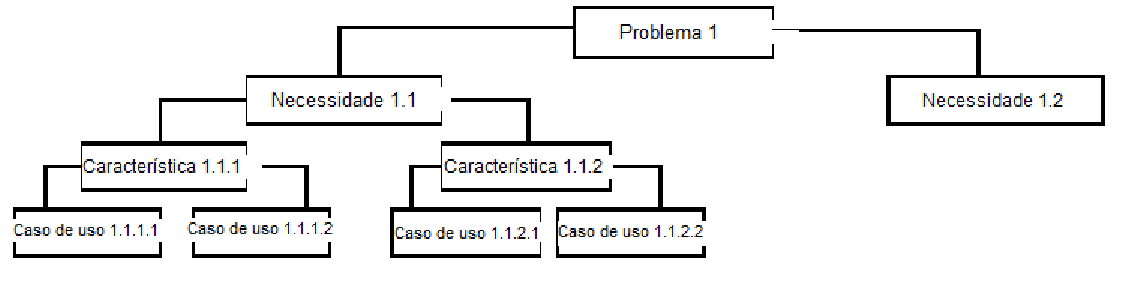
\includegraphics[width=0.8\textwidth]{imgModelagem/diagrama}
	\caption{Matriz de rastreabilidade}
	\label{img:rastreabilidade}
\end{figure}


%-----------------------------------------------------------------------------------------------------------
\subsection{Descrições da Parte Interessada e do Usuário}

Nesta sessão serão identificados e detalhados os interessados e usuários da \nomeferramenta{}.

\subsubsection{Resumo da Parte Interessada e do Usuário}

Para melhor entendimento das características e responsabilidades dos interessados, utilizou-se uma tabela que apresenta todos os interessados no sistema, suas descrições, responsabilidades e os critérios de sucesso de suas funções na equipe, ilustrada na tabela \ref{tab:parteInteressada}. Com esta tabela, pode-se obter o entendimento necessário sobre os interessados e o quão importante eles são para o sucesso do sistema.

\begin{table}[htbp]
\centering
\begin{tabular}{|p{2cm}|p{5cm}|p{4cm}|p{4cm}|}
\hline
%-------------------------------------------------------
\textbf{Interessado} &
\textbf{Descrição} &
\textbf{Responsabilidade} &
\textbf{Critérios de Sucesso}
\\ \hline

%-------------------------------------------------------
Analista de Requisitos &
Membro da equipe de desenvolvimento com facilidade em comunicação, psicologia, sociologia, filosofia e mais áreas que possam facilitar a relação com o cliente. Seu conhecimento na área pode ser, dependendo da organização, baixo. &
Pessoa responsável por realizar a elicitação dos requisitos junto ao usuário. Deve elicitar os requisitos de forma adequada à garantir sucesso no desenvolvimento do \sw. &
Requisitos corretamente elicitados e prontos para serem documentados. 
\\ \hline
%-------------------------------------------------------
Gerente de Requisitos &
Conhecedor de todo o processo de desenvolvimento e com contato frequente com o cliente. Seu conhecimento deve ser alto. &
Pessoa responsável por administrar os requisitos durante todo processo de desenvolvimento de \sw, garantindo o mínimo esforço em casos de mudança de requisitos. &
Requisitos bem administrados para, no caso de mudanças nos requisitos, existir o menor impacto possível na equipe de desenvolvimento.
\\ \hline
%--------------------------------------------------------
\end{tabular}
\label{}
\caption{Parte Interessada}
\label{tab:parteInteressada}
\end{table}

\subsubsection{Principais Problemas e Necessidades da Parte Interessada}

O problema a ser resolvido pela \nomeferramenta~ deve estar bastante claro entre todos os \stakeholder~ para que o desenvolvimento passe pela menor quantidade possível de dificuldades quanto ao entendimento de onde focar esforços para desenvolver a solução do problema.

Para o mapeamento do problema principal e suas causas, foi utilizada a técnica de \textit{fishbone}. Segue o resultado da mesma na figura \ref{img:fishbone}

%-------------------------------------FISHBONE AQUI----------------------------------------
\begin{figure}[H]
	\centering
	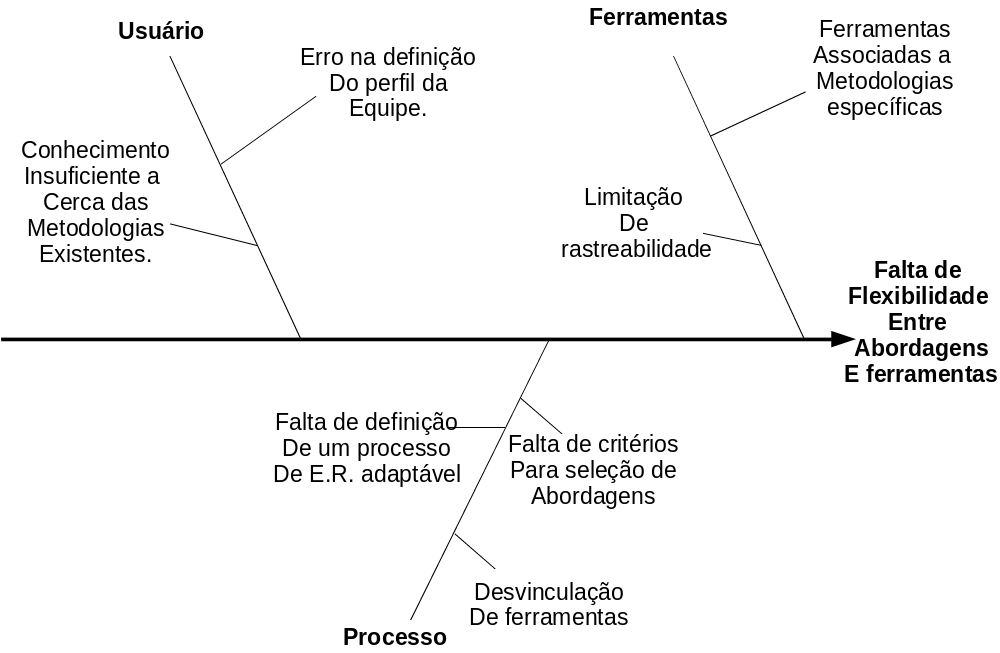
\includegraphics[width=0.8\textwidth]{imgModelagem/fishbone}
	\caption{Fishbone de Problema}
	\label{img:fishbone}
\end{figure}
%-------------------------------------FISHBONE AQUI----------------------------------------

Para melhor entendimento do problema, utilizamos a técnica de \textit{Framework de problema}, que consiste em criar uma tabela apresentando o problema, os afetados, o impacto do problema e qual seria uma solução bem sucedida, o Framework esta retratado na tabela \ref{tab:frameworkproblema}.

\begin{table}[htbp]
\centering
\begin{tabular}{|p{2.5cm}|p{10cm}|p{2.5cm}|}
%----------------------------------------------
\hline
\textbf{O Problema:} &
Dificuldade no Gerenciamento de requisitos em processos flexíveis. 
\\ \hline
%----------------------------------------------
\textbf{Afeta:} &
Todos os desenvolvedores de \sw~ que necessitam de uma flexibilidade maior na gerência de requisitos.
\\ \hline
%----------------------------------------------
\textbf{Cujo impacto é:} &
Processo de requisitos mal gerenciados, aumentando a possibilidade de erros durante o desenvolvimento.
\\ \hline
%----------------------------------------------
\textbf{Uma solução bem sucedida seria:} &
Utilização de uma ferramenta que faça gerência de requisitos de forma flexivel, podendo utilizá-la em qualquer metodologia.
\\ \hline
%----------------------------------------------
\end{tabular}
\caption{Framework de Problema}
\label{tab:frameworkproblema}
\end{table}

Após o entendimento do problema, vê-se necessária a documentação das necessidades do cliente. Utilizou-se de uma técnica chamada \textit{framework de necessidades} na qual são apresentados todos os problemas, as necessidades, a solução atual e a solução proposta. Dessa forma, pode-se obter um entendimento mais organizado dos problemas e necessidades do cliente, de acordo com o retradado na tabela \ref{tab:frameworknecessidade}.

\begin{table}[H]
\centering
\begin{tabular}{|p{5cm}|p{3cm}|p{3cm}|p{5cm}|}

%-------------------------------------------------------------
\hline
\textbf{Necessidade} &
\textbf{Problema} &
\textbf{Solução Atual} &
\textbf{Solução Proposta}
\\ \hline
%-------------------------------------------------------------
Descobrir a metodologia ideal a ser utilizada no projeto. &
Utilização de metodologias que não se adéquam as características do projeto. &
A equipe de desenvolvimento escolhe a sua metodologia. &
Criação de uma ferramenta que apresente a melhor opção de metodologia a ser seguida, de acordo com as características do projeto, equipe e cliente.
\\ \hline
%-------------------------------------------------------------
Obter a metologia que melhor se adequa ao contexto, mesmo sem ter conhecimento profundo sobre a mesma. &
Conhecimento insuficiente a cerca das metodologias existentes. &
Estudar as metodologias existentes. &
Criação de uma ferramenta que faça a seleção da melhor metodologia sem que os envolvidos precisem ter conhecimento sobre a mesma.
\\ \hline
%-------------------------------------------------------------
Criação de uma rastreabilidade de fácil entendimento e bem organizada. &
Dificuldade em manter rastreabilidades de requisitos. &
Realizar a rastreabilidade a partir do conhecimento da equipe. &
Utilização de uma ferramenta que documente os requisitos tomando cuidado com a rastreabilidade do mesmo, garantindo organização e fácil entendimento. 
\\ \hline
%-------------------------------------------------------------
Necessidade de ferramentas flexíveis, que utilizam determinada metodologia de acordo com as características do projeto. &
Ferramentas existentes direcionadas a apenas uma metodologia. &
Utilização de mais de uma ferramenta em diferentes projetos. &
Criação de uma ferramenta que se adeque a todas as metodologias,de acordo com as características do projeto. 
\\ \hline
%-------------------------------------------------------------
Obter o perfil da equipe já definido. &
Erro na definição do perfil da equipe. &
A própria equipe define seu perfil. &
Criação de uma ferramenta que apresente o perfil da equipe a partir de \textit{inputs} que representam algumas características da mesma.
\\ \hline
%-------------------------------------------------------------
\end{tabular}
\caption{Framework de Necessidades}
\label{tab:frameworknecessidade}
\end{table}

%-----------------------------------------------------------------------------------------------------------
\subsection{Visão Geral do Produto}
	
Nesta seção, pode-se ter um entendimento geral de como será o produto final, quais serão suas características, como serão suas funcionalidades e etc.

\subsubsection{Perspectiva do Produto}
	
O produto se encontrará em um contexto onde existem inúmeras ferramentas com o mesmo propósito, porém, as ferramentas existentes são inflexíveis quando se trata da abordagem que será seguida durante o desenvolvimento de \sw. Esta falha será corrigida na \nomeferramenta, que irá propor uma metodologia para cada projeto em particular de acordo com suas características.

A ferramenta pode ser autocontida, não necessitando do apoio de nenhum outro sistema, porém a utilização de ferramentas de modelagem de processos é bastante indicada para que a máxima organização do projeto seja alcançada.

\subsubsection{Resumo das Capacidades}
	
O grande diferencial da \nomeferramenta~ será a flexibilização na abordagem que será seguida durante o gerenciamento de projetos de \sw. O sistema deverá indicar a melhor abordagem a ser seguida pela equipe de desenvolvimento, garantindo a otimização do processo de desenvolvimento.

A ferramenta será capaz de disponibilizar a opção de modificar a abordagem indicada pela ferramenta, para que a equipe de desenvolvimento possa escolher a abordagem na qual os mesmos se sentem mais a vontade.

%-----------------------------------------------------------------------------------------------------------
\subsection{Recursos do Produto}
%Lista e descreve brevemente os recursos do produto. Os recursos são capacidades de alto nível do sistema que são necessários para entregar benefícios aos usuários. Cada recurso é um serviço solicitado que, em geral, requer uma série de entradas para alcançar o resultado desejado. Por exemplo, um recurso de um sistema de rastreamento de problemas pode ser a capacidade de fornecer relatórios de tendências. À medida que o modelo de casos de uso toma forma, atualize a descrição para fazer referência aos casos de uso.

%Como o documento de visão é revisado por uma ampla variedade de equipes envolvidas, mantenha o nível de detalhes gerais suficiente para que todos possam entender. No entanto, ofereça detalhes suficientes para fornecer à equipe as informações que ela precisa para criar um modelo de casos de uso ou outros documentos de design.

%Para gerenciar a complexidade do aplicativo, para um novo sistema ou uma mudança incremental, liste os recursos em um alto nível para que você possa incluir aproximadamente 25 a 99 recursos. Esses recursos fornecem a base para a definição do produto, gerenciamento de escopo e gerenciamento do projeto. Cada recurso será expandido mais detalhadamente no modelo de casos de uso.

%Em toda esta seção, torne cada recurso relevante para usuários, operadores ou outros sistemas externos. Inclua uma descrição de funções e problemas de usabilidade que devem ser tratados. As seguintes diretrizes se aplicam:
%Evite design. Mantenha as descrições do recurso em um nível geral. Foque nas capacidades necessárias e por que (não como) elas devem ser implementadas.
%Designe todos os recursos como requisitos de um tipo de recurso específico para fácil referência e rastreamento.

\subsubsection{Recurso 1}

\subsubsection{Recurso 2}

%-----------------------------------------------------------------------------------------------------------
\subsection{Restrições}

O sistema operacional poderá ser Windows e algumas destribuições de linux como Ubuntu, mint e open suse, o software também poderá ser executado pelos navegadores Google Chrome, Fire fox e só não será viavel sua utilização no Internet Explorer e Safari.
%Observe todas as restrições de design, restrições externas, como requisitos operacionais ou regulamentares) ou outras dependências.

%-----------------------------------------------------------------------------------------------------------
\subsection{Faixas de Qualidade}
%Defina as faixas de qualidade para desempenho, robustez, tolerância a falhas, usabilidade e características similares que o conjunto de recursos não descreve.


%-----------------------------------------------------------------------------------------------------------
\subsection{Precedência e Prioridade}
%Define a prioridade dos diferentes recursos do sistema.

%-----------------------------------------------------------------------------------------------------------
\subsection{Outros Requisitos do Produto}
%Em um alto nível, lista os padrões aplicáveis, os requisitos de hardware ou plataforma, os requisitos de desempenho e os requisitos ambientais.

\subsubsection{Padrões Aplicáveis}
%Lista todos os padrões que o produto deve estar em conformidade. A lista pode incluir estes padrões:
%Padrões jurídicos e regulamentares (FDA, UCC)
%Padrões de comunicações (TCP/IP, ISDN)
%Padrões de conformidade da plataforma (Windows, UNIX, etc.)
%Padrões de qualidade e segurança (UL, ISO, CMM)

\subsubsection{Requisitos do Sistema}
%Define os requisitos do sistema para o aplicativo. Eles incluem os sistemas operacionais do host suportados e as plataformas de rede, configurações, memória, dispositivos periféricos e software de parceiros.

\subsubsection{Requisitos de Desempenho}
%Detalha os requisitos de desempenho. Os problemas de desempenho podem incluir itens como fatores de carga do usuário, largura de banda ou capacidade de comunicação, rendimento, exatidão, confiabilidade ou tempos de resposta em uma variedade de condições de carregamento.

\subsubsection{Requisitos Ambientais}
%Detalha os requisitos ambientais conforme necessário. Para sistemas baseados em hardware, os problemas ambientais podem incluir temperatura, choque elétrico, umidade e radiação. Para aplicativos de software, os fatores ambientais podem incluir condições de uso, ambiente do usuário, disponibilidade do recurso, problemas de manutenção, manipulação de erros e recuperação.

%-----------------------------------------------------------------------------------------------------------
\subsection{Requisitos de Documentação}
%Esta seção descreve a documentação que deve ser desenvolvida para suportar a implementação bem sucedida do aplicativo.

\subsubsection{	Notas sobre a liberação, arquivo Leia-me}
%As notas sobre a liberação ou um arquivo Leia-me abreviado podem incluir uma seção "O que Há de Novo", uma discussão sobre problemas de compatibilidade com liberações anteriores, e alertas de instalação e atualização. O documento pode também conter ou vincular correções na liberação e quaisquer problemas ou soluções alternativas conhecidos.

\subsubsection{Ajuda On-line}
%Muitos aplicativos fornecem um sistema de ajuda on-line para ajudar o usuário. A natureza desses sistemas é exclusiva para desenvolvimento de aplicativo, pois eles combinam aspectos de programação (centros de informações pesquisáveis e navegação do tipo Web) com aspectos de composição técnica (organização, apresentação). Muitas equipes consideram que o desenvolvimento do sistema de ajuda on-line é um projeto dentro de um projeto que se beneficia do gerenciamento de escopo e planejamento no início do projeto.

\subsubsection{Guias de Instalação}
%Um documento que inclui instalação, configuração e instruções de atualização como parte da oferta de solução integral.

%-----------------------------------------------------------------------------------------------------------
\subsection{Atributos do Recurso}
%Fornece aos recursos atributos que podem ser usados para avaliar, controlar, priorizar e gerenciar os itens de produtos propostos para implementação. Descreve todos os tipos de requisitos e atributos em um plano de gerenciamento de requisitos. No entanto, você pode listar e descrever brevemente os atributos para os recursos que foram escolhidos. As subseções a seguir representam um conjunto de atributos de recursos sugeridos.

\subsubsection{Status}
%Aqui inserir a tabela que esta no doucmento antigo.

\subsubsection{Prioridade}

\subsubsection{Arquitetura}